\subsection{Richards Frequenztransformation}

Der  Frequenzbereich von konzentrierten LC-Filtern ist beschr\"ankt durch  die
Nichtidealit\"at der Komponenten.  W\"ahrend  die  Reaktanz und die G\"ute von
konzentrierten Induktivit\"aten und Kapazit\"aten  im  Bereich  \"uber  einige
\SI{100}{\mega\hertz} keinen hohen Filteranspr\"uchen mehr gen\"ugen k\"onnen,
w\"aren die entsprechenden Reaktanzen noch  sehr gut mit verteilten Elementen,
wie   leerlaufenden   und   kurzgeschlossenen  Leitungen  sowie  verschiedenen
gekoppelten   Leitungen  realisierbar.   Es   ist   beispielsweise   aus   der
Leitungstheorie  bekannt,  dass  leerlaufende  Leitungen   mit  einer  L\"ange
$l\le\frac{\lambda}{4}$   kapazitiv   und   kurzgeschlossene   Leitungen   mit
$l\le\frac{\lambda}{4}$  induktiv  sind.  Wir  k\"onnten damit die  induktiven
Reaktanzen und  die  kapazitiven  Suszeptanzen  mit  solchen Leitungselementen
ersetzen.

Eine Methode dies zu  erreichen  ist mithilfe der sogenannten \textit{Richards
Frequenztransformation}.   Dabei   ist   wichtig   zu   beachten   dass   alle
Leitungselemente  die  gleiche  L\"ange   $l$  haben  m\"ussen.  Sie  hat  die
allgemeine Form:

\begin{equation}
    \Omega = \frac{\Omega'}{\Omega'_c} = \frac{1}{\Omega'_c}\tan\frac{\pi f}{2f_0}
    \label{eq:richards}
\end{equation}

Dabei sind

\begin{align*}
    \Omega &: \textrm{normierte Frequenz des konzentrierten Netzwerkes} \\
    \Omega' &: \textrm{reelle normierte Frequenz}\hspace{5mm}\Omega' = \tan\frac{\pi f}{2f_0} \\
    \Omega'_c &: \textrm{reelle normierte Durchlassfrequenz}\hspace{5mm}\Omega'_c = \tan\frac{\pi f_c}{2f_0}
\end{align*}

F\"ur die Leitungselemente des Filters gelten

\begin{align}
    j\Omega\omega_cL_i &= jZ_{w_i}\tan\frac{\pi f}{4f_c} \\
    j\Omega\omega_cC_i &= jY_{w_i}\tan\frac{\pi f}{4f_c}
\end{align}

Dabei sind

\begin{tabular}{ll}
    $L_i$ und $C_i$         & die Induktivit\"aten und Kapazi\"aten des \\
                            & konzentrierten Filters. \\
    $Z_{w_i}$ und $Y_{w_i}$ & die Wellenimpedanzen und Wellenadmittanzen \\
                            & der kurzgeschlossenen und leerlaufenden \\
                            & Leitungen des Leitungsfilters. \\
\end{tabular}

Zur Visualisierung wurde mit MATLAB der  Amplitudengang  $T(s)$ eines analogen
Chebychev-Fiefpassfilters 3.  Ordnung  mit  der  Formel  $s  =  j\tan\frac{\pi
\omega}{2\omega_0}$ (Formel \ref{eq:richards}) transformiert. Das Resultat ist
in der Abbildung \ref{fig:richards-example} zu sehen.

\begin{figure}[h!]
    \centering
    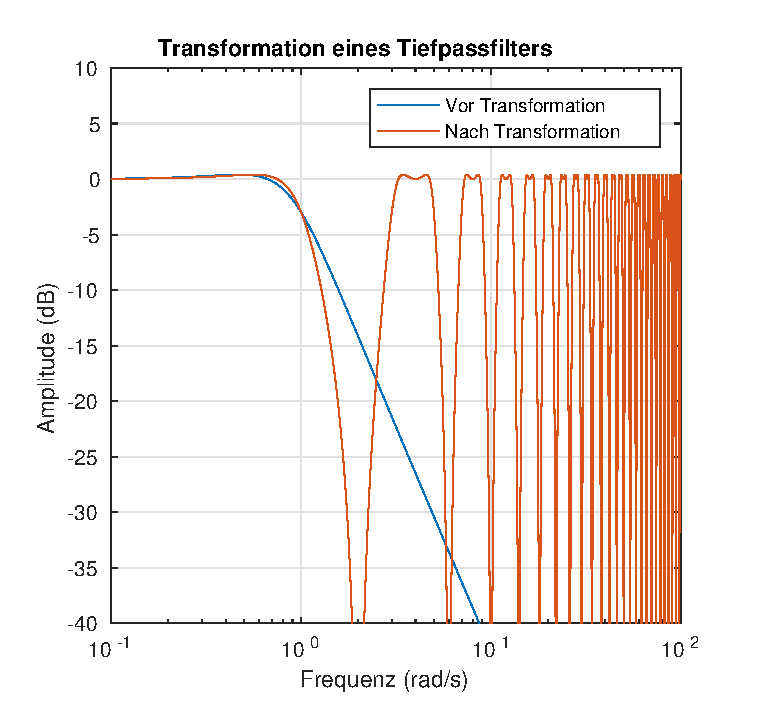
\includegraphics[width=\imagewidth]{images/richards-lowpass-example}
    \caption{Chebychev-Tiefpassfilters 3. Ordnung (blau) und die Richards-Transformierte davon (orange)}
    \label{fig:richards-example}
\end{figure}

Die  D\"ampfungscharakteristik  des   Leitungsfilters  weist  gegen\"uber  dem
konzentrierten  LC-Filter eine verzerrte Frequenzskala auf und ist  periodisch
mit der Periodizit\"at

\begin{equation}
    4f_c = \frac{\nu_p}{2l}
\end{equation}

Wobei $\nu_p$ die Phasengeschwindigkeit auf der Leitung ist.

Die Periodizit\"at war  zu  erwarten,  da  alle Leitungenselemente die gleiche
L\"ange $l$ haben und so eine ortsabh\"angige wiederholung der Phase bewirken.
Unerw\"unschte Durchlassbereiche bei  h\"oheren Frequenzen k\"onnen anhand von
in Kaskade geschaltenen Filtern mit unterschiedlich  hohen  Durchlassbereichen
unterdr\"uckt werden.

\begin{figure}[h!]
    \centering
    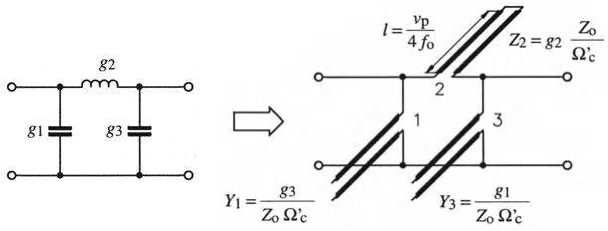
\includegraphics[width=\imagewidth]{images/LC-zu-Leitungsfilter}
    \caption{Realisierung von Stichleitungen in Mikrostreifentechnik, Auszug aus dem Buch Mikrowellentechnik\cite[p.~26]{ref:baechold}}
    \label{fig:LC-zu-Leitungsfilter}
\end{figure}

